\documentclass[a4j]{ujarticle}
\usepackage[dvipdfmx]{graphicx}
\usepackage{url}
\usepackage{bbding}
\usepackage{lscape}
\usepackage[subrefformat=parens]{subcaption}
\usepackage{bm}
\usepackage{amsmath}

\title{ミーティング資料}
\author{安達智哉\\to-adachi@ist.osaka-u.ac.jp}
\date{2019年4月24日}

\begin{document}
\maketitle


\section{シグナリング数の調査結果}
\label{sec:signalings}
先行研究を調査することにより、状態遷移に伴うシグナリングの発生数が一部であるが、明らかになった。
図\ref{state_id}に示す状態遷移図と共に、状態遷移に伴って発生するシグナリングに関する情報を、表\ref{table:signalings_all}に示す。

\begin{figure}[htbp]
  \centering
  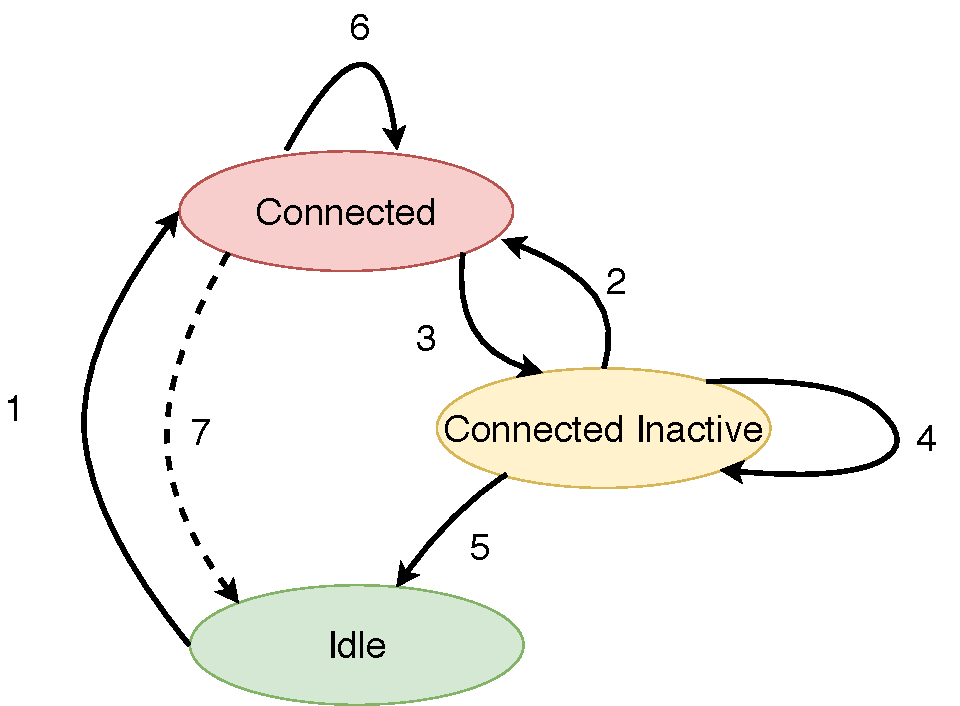
\includegraphics[width=0.9\hsize]{state_id.pdf}
  \caption{state transition}
  \label{state_id}
\end{figure}

\begin{table}[htbp]
  \centering
  \caption{Signaling Load}
  \label{table:signalings_all}
  \begin{tabular}{c|cccc|l}
    \hline
    遷移ID  & \multicolumn{4}{|c|}{シグナリング処理数} & 遷移条件                          \\
            & UE      & RAN     & MME     & SGW      &                                   \\ \hline \hline
    1       & 9       & 12      & 5       & 2        & Packets transmission              \\
    2       & 5       & 5       & 0       & 0        & 2 or more packets transmission    \\
    3       & 1       & 1       & 0       & 0        & Connected timer expiration        \\
    4       & 4       & 4       & 0       & 0        & One packet transmission           \\
    5       & 0       & 3       & 5       & 2        & Connected Inactive timer expiration             \\
    6       & 0       & 0       & 0       & 0        & Packets transmission              \\
    7       & 1       & 4       & 5       & 2        & Connected timer expiration            \\ \hline
  \end{tabular}
\end{table}

\clearpage
\section{メモリ負荷の算出}
% 第\ref{sec:signalings}章の調査結果より、Connected状態とConnected Inactive状態間の状態遷移の際にはMMEおよびSGWにはシグナリングが発生しないことが明らかになった。
% シグナリングが発生していないことから、MMEおよびSGWで保持している情報にも変化がないと推定できる。
% そのため、これらのノードのメモリ負荷はConnected状態とConnected Inactive状態で同じであると考えられる。
% その上で、Idle状態からConnected状態に遷移した際に、MMEにどれほどのMME負荷が発生するのかを調査してきた。

文献\cite{3gpp.23.720}に示されている、コネクション確立に伴うシグナリング図を図\ref{Legacy_connection_setup}に示す。
この図を見るとUEがIdle状態からConnected状態へ遷移する際に、様々なシグナリングが発生していることがわかる。
これらのシグナリングにどのような情報が含まれているかを調査することにより、各ノードが保持する情報を知ることができると考えられる。
そのため今回は、これらのシグナリングの内、MMEが関与しているシグナリングについて、文献\cite{3gpp.36.413}および文献\cite{3gpp.29.274}を参考にして調査を行った。
\begin{figure}[htbp]
  \centering
  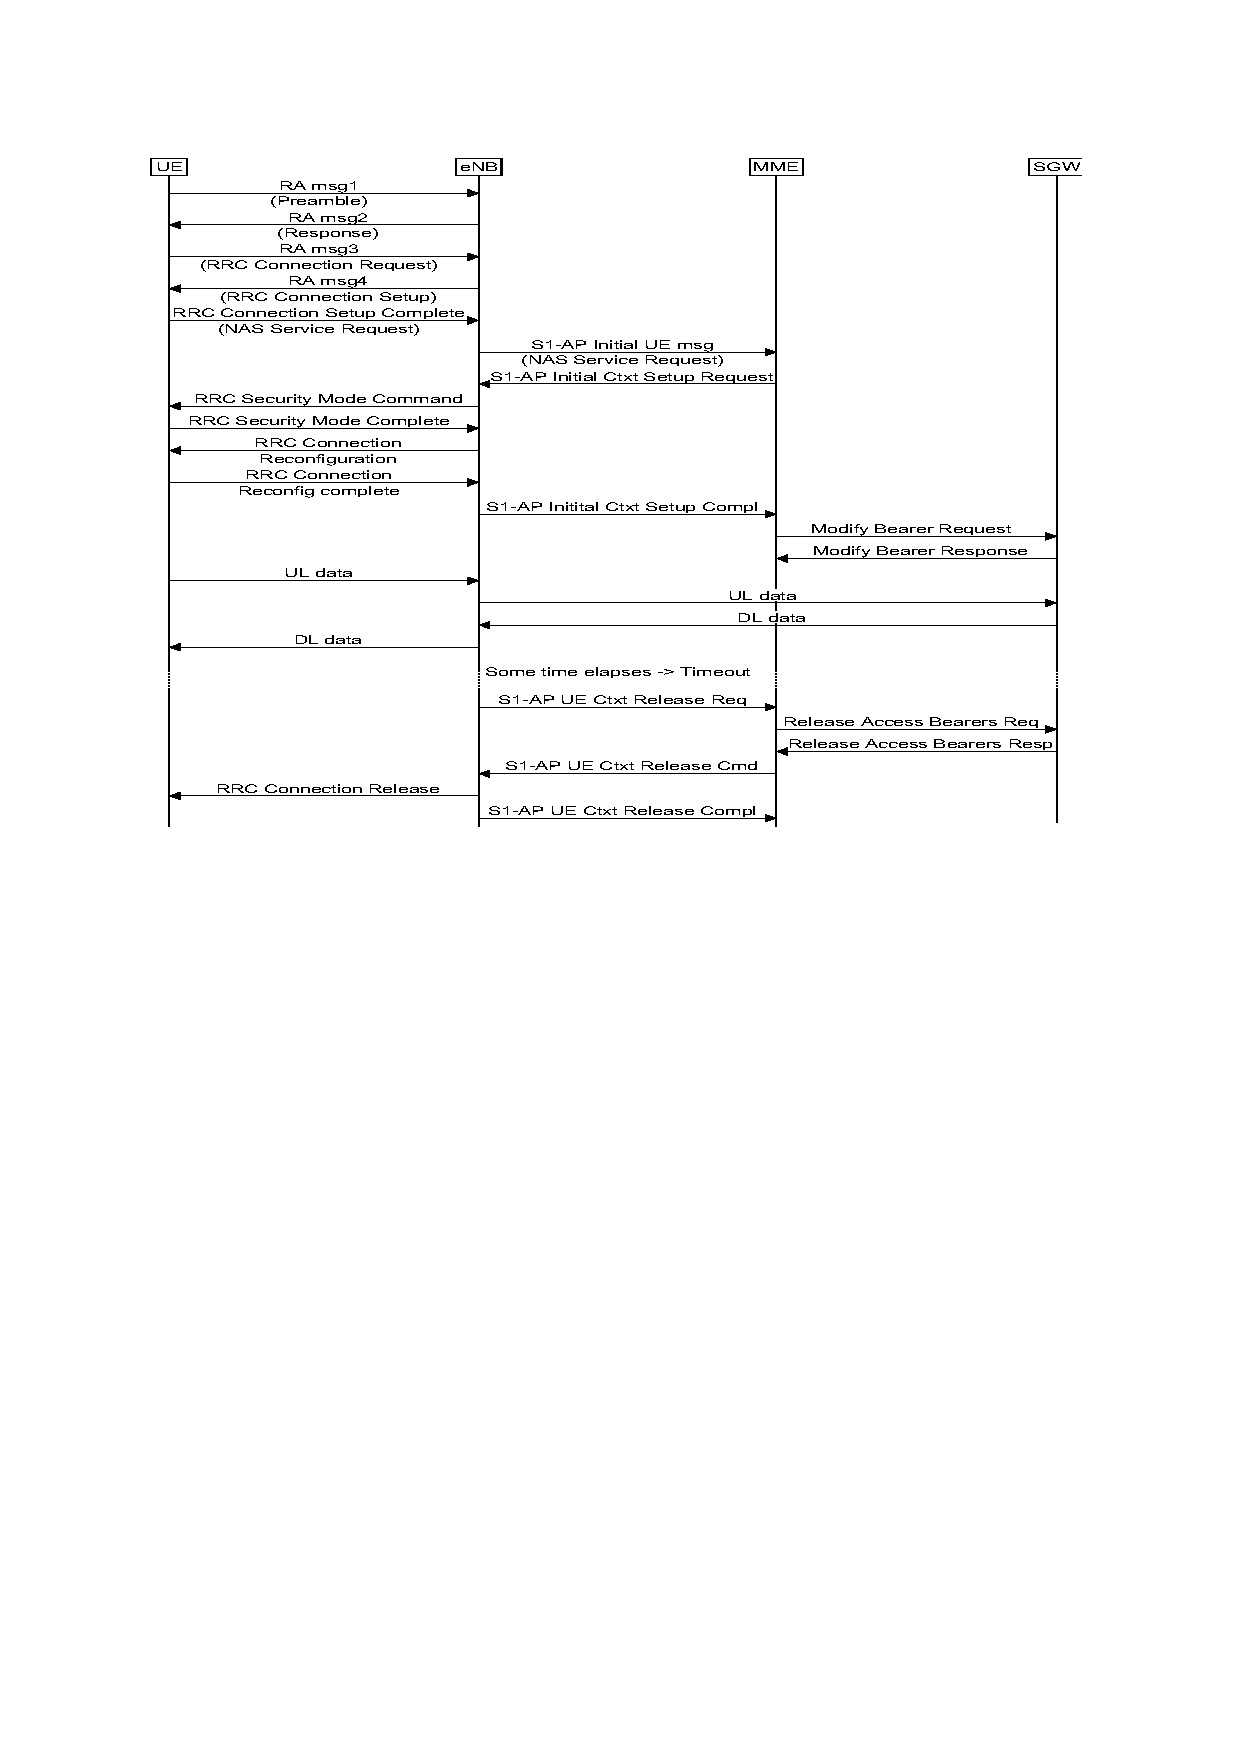
\includegraphics[width=0.9\hsize]{Legacy_connection_setup.pdf}
  \caption{Legacy connection setup}
  \label{Legacy_connection_setup}
\end{figure}


\subsection{SI-AP Initial UE msg}
SI-AP Initial UE msgに含まれる情報を以下に示す。
\begin{itemize}
  \item NAS メッセージ
  \item eNB UE S1AP ID
\end{itemize}
この文献に明記されている訳ではないが、おそらくMMEはこれらの情報保持するのではないかと考えられる。


\subsection{SI-AP Initial Ctxt Setup Request/Complete}
SI-AP Initial Ctxt Setup Requestメッセージに含めてる情報を以下に示す。
\begin{itemize}
  \item the Handover Restriction List IE, which may contain roaming or access restrictions.
  \item the UE Radio Capability IE.
  \item the Subscriber Profile ID for RAT/Frequency priority IE.
  \item the SRVCC Operation Possible IE.
  \item the UE Sidelink Aggregate Maximum Bit Rate IE.
  % ここまでは明記 以下は少し怪しい
  \item NAS-PDU IE
  \item the Trace Activation IE.
  \item the CSG Membership Status IE.
  \item the Management Based MDT PLMN List IE.
  \item the Additional CS Fallback Indicator IE.
  \item the ProSe Authorized IE.
  \item the V2X Services Authorized IE.
\end{itemize}
% また、オプションもしくは特定の条件下のみで以下の情報をメッセージに含むことができる。
% \begin{itemize}
%   \item the Correlation ID IE in case of LIPA operation
%   \item the SIPTO Correlation ID IE in case of SIPTO@LN operation
%   \item the Bearer Type IE
%   \item the CS Fallback Indicator IE.
%   \item the Registered LAI IE.
%   \item the GUMMEI IE, which indicates the MME serving the UE.
%   \item the MME UE S1AP ID 2 IE, which indicates the MME UE S1AP ID assigned by the MME
%   \item the Management Based MDT Allowed IE.
%   \item the Masked IMEISV IE.
%   \item the Expected UE Behaviour IE.
%   \item the UE User Plane CIoT Support Indicator IE.
%   \item the NR UE Security Capabilities IE.
%   \item the Aerial UE subscription information IE.
%   \item the Pending Data Indication IE.
% \end{itemize}
また、eNodeBはSI-AP Initial Ctxt Setup Requestメッセージを受信した上で、以下の情報を保持する。
\begin{itemize}
  \item UE Aggregate Maximum Bit Rat
  \item Handover Restriction List
  \item UE Radio Capability
  \item Subscriber Profile ID for RAT/Frequency priority
  \item SRVCC Operation Possible
  \item UE Security Capabilities
  \item Security Key
\end{itemize}
% また、以下の情報をオプションもしくは特定の条件下のみで保持する。
% \begin{itemize}
%   \item CSG Membership Status (if supported)
%   \item Management Based MDT Allowed information (if supported)
%   \item Management Based MDT PLMN List information (if supported)
%   \item ProSe Authorization information (if supported)
%   \item V2X Services Authorization information (if supported)
%   \item UE Sidelink Aggregate Maximum Bit Rate (if supported)
% \end{itemize}

eNBは、INITIAL CONTEXT SETUP RESPONSEメッセージを用いて、UEとのセキュリティ手順の確立に成功したこと、および要求されたすべてのeNodeB-Radio Access Bearerの結果をMMEに報告する。 具体的には以下の情報をINITIAL CONTEXT SETUP RESPONSEに含める。
\begin{itemize}
  \item A list of E-RABs which are successfully established shall be included in the E-RAB Setup List IE
\end{itemize}
こちらに関しても文献に明記されている訳ではないが、MMEはこれらの情報保持するのではないかと考えられる。
\subsection{modify bearer request/response}
modify bearer requestには以下の情報が含まれる。
\begin{itemize}
  \item Sender F-TEID for Control Plane
  \item Aggregate Maximum Bit Rate (APN-AMBR)
  \item Delay Downlink Packet Notification Request
  \item Bearer Contexts to be modified
  \item MME-FQ-CSID
  \item SGW-FQ-CSID
\end{itemize}
また、modify bearer responseには以下の情報が含まれる。
\begin{itemize}
  \item APN Restriction
  \item Bearer Contexts modified
  \item PGW-FQ-CSID
  \item SGW-FQ-CSID
\end{itemize}
こちらに関しても文献に明記されている訳ではないが、MMEはこれらの情報保持するのではないかと考えられる。
\subsection{S1-AP UE Context release request/command/complete}
S1-AP UE Context release requestには、S1コネクションを解放するための適切な原因を示す情報が含まれている。
私の研究で想定している環境においては、以下の情報が含まれることになる。
\begin{itemize}
  \item User Inactivity
\end{itemize}
S1-AP UE Context release commandには以下の情報が含まれる。
S1-AP UE Context release commandを受け取ったeNodeBは、関連するシグナリングおよびユーザデータ転送リソースを解放する。
その後、S1-AP UE Context release completeメッセージをMMEに送信する。
\begin{itemize}
  \item MME UE S1AP ID IE
  \item cause IE
\end{itemize}

\subsection{release access bearer request/response}
文献\cite{3gpp.29.274}によると、release access bearer requestには以下の情報が含まれる。
\begin{itemize}
  \item List of RABs
\end{itemize}
また、release access bearer responseには以下の情報が含まれる。
\begin{itemize}
  \item Cause
\end{itemize}


\subsection{現段階での考察}
今回はMMEに着目し、Connected状態およびIdle状態を遷移する際にMMEがどのような情報を扱っているのかを明らかにすることができた。
これらの情報はいずれもUEが通信を行うために必要なものであると考えられるため、UEがConnected状態である時は、MMEはこれらの情報を保持すると考えられる。
よって、MMEのメモリ負荷を推定する際に、参考にすることができると思う。
また、前回の進捗報告でも述べたが、各シグナリングメッセージにはオプションの項目が数多く用意されており、ネットワークの構成や状態に依存してシグナリングに含まれる情報が変動する可能性があることを留意するべきである(今回はオプションの情報は考慮していない)。
\section{今後の課題}
  \begin{itemize}
    \item 状態遷移に伴って発生するシグナリングの調査。
    \item Connected Inactive状態において``状態遷移を伴わないデータ送信"が可能なデータ量の調査。
    \item メモリ負荷の算出
  \end{itemize}

\section*{\addcontentsline{toc}{section}{参考文献}}
\bibliographystyle{IEEEtran}
\bibliography{/Users/t-adachi/Documents/study/Bibliography/bib/hpt_core_network/myBib/LABbiblio,/Users/t-adachi/Documents/study/Bibliography/bib/hpt_core_network/Study_Group_Bibtex/bib/hptCoreNetwork_Study}
\end{document}
